% Chapter 4
\section[Gradient descent: iteration and exact solutions]{Gradient Descent, the Optimization View: Iteration, Fixed Points, and an Exact Solution}\label{sec:gd}

Section~\ref{sec:hd-closed} gave the closed-form solution $\bhat = (\X^\top\X)^{-1}\X^\top\y$, but ``can be written down'' is not ``should be computed that way'': explicit inversion solves a $d \times d$ linear system at cost $O(d^3)$, and forming $\X^\top\X$ squares the condition number of $\X$. This chapter switches to the optimization view: instead of solving the normal equations directly, start from some $\widehat{\bbeta}_0$ and let the loss function ``walk downhill.'' We will see — \textbf{because the loss is quadratic, this downhill path can be written down exactly}: $\widehat{\bbeta}_t$ has a closed-form expression in $t$, $\X$, and $\y$, and its fixed point is precisely the closed-form solution $\bhat$.

\subsection{The Gradient Descent Iteration and Its Fixed Point}\label{sec:gd-iter}

Adopt the standard convention from machine learning:
\begin{equation}\label{eq:gd-loss}
  L(\bbeta) = \frac{1}{2}\norm{\y - \X \bbeta}^2,
  \qquad
  \nabla L(\bbeta) = \X^\top (\X \bbeta - \y),
\end{equation}
(the $\frac12$ is only a convention so that the gradient carries no factor $2$; if you insist on $L = \norm{\cdot}^2$, replace every $\eta$ below by $2\eta$.) Note that the iteration as first written,
\[
  \widehat{\bbeta}_{t+1} = \widehat{\bbeta}_t - \eta\, L(\widehat{\bbeta}_t),
\]
needs a small correction: $L$ is a scalar, and a scalar cannot be subtracted from a vector — the downhill direction is the \textbf{negative gradient}, with step size (learning rate) $\eta > 0$:
\begin{equation}\label{eq:gd}
  \boxed{\;\widehat{\bbeta}_{t+1} = \widehat{\bbeta}_t - \eta\, \nabla L(\widehat{\bbeta}_t)
       = \widehat{\bbeta}_t - \eta\, \X^\top \big( \X \widehat{\bbeta}_t - \y \big)\;}
\end{equation}

A \textbf{fixed point} is one that stops moving after an iteration step:
\begin{equation}\label{eq:fixed}
  \bbeta^\star = \bbeta^\star - \eta\, \nabla L(\bbeta^\star)
  \quad\Longleftrightarrow\quad
  \nabla L(\bbeta^\star) = \zero
  \quad\Longleftrightarrow\quad
  \X^\top \X \, \bbeta^\star = \X^\top \y .
\end{equation}
The fixed-point condition \emph{is} the normal equation! So when $\X$ has full column rank and $0 < \eta < \infty$, \eqref{eq:gd} has the unique fixed point
\begin{equation}\label{eq:gd-fixed}
  \boxed{\;\bbeta^\star = (\X^\top \X)^{-1} \X^\top \y = \bhat\;}
\end{equation}
Gradient descent and least squares are two paths to the same object: \textit{one solves the equations directly (Section~\ref{sec:hd-closed}), the other iterates toward them (this section) — and they share the same destination.} This is the first layer of ``putting the two formulas together.''

\subsection[Putting the Two Formulas Together: The Exact Solution for the Iterate]{Putting the Two Formulas Together: An Exact Solution for $\widehat{\bbeta}_t$}\label{sec:gd-exact}

Now for the second layer: combine \eqref{eq:gd} with \eqref{eq:gd-fixed} to write the \textbf{exact solution at any time $t$}.

Rewrite \eqref{eq:gd} in ``error propagation'' form. Let $\bm{A} := \bm{I} - \eta \X^\top \X$; the fixed point gives
\[
  \eta\, \X^\top \y = \eta\, \X^\top \X \bbeta^\star = (\bm{I} - \bm{A})\, \bbeta^\star .
\]
Substituting into \eqref{eq:gd}:
\[
  \widehat{\bbeta}_{t+1} = (\bm{I} - \eta \X^\top\X)\, \widehat{\bbeta}_t + \eta \X^\top \y
  = \bm{A}\, \widehat{\bbeta}_t + (\bm{I} - \bm{A})\, \bbeta^\star,
\]
i.e.
\[
  \widehat{\bbeta}_{t+1} - \bbeta^\star = \bm{A}\, \big( \widehat{\bbeta}_t - \bbeta^\star \big).
\]
The error vector is multiplied by the same matrix $\bm{A}$ at every step — the entire secret of linear iteration lives in this line. Unrolling $t$ times:

\begin{theorem}[Exact solution for $\widehat{\bbeta}_t$]\label{thm:gd-exact}
For any initialization $\widehat{\bbeta}_0$ and any $t \ge 0$,
\begin{equation}\label{eq:gd-exact}
  \boxed{\;\widehat{\bbeta}_t = \underbrace{(\X^\top \X)^{-1} \X^\top \y}_{\bhat}
  + \big( \bm{I} - \eta\, \X^\top \X \big)^{t}\; \big( \widehat{\bbeta}_0 - (\X^\top \X)^{-1} \X^\top \y \big)\;}
\end{equation}
``closed-form solution $+$ $t$-th power decay of the initial error.'' In particular, with the most common default $\widehat{\bbeta}_0 = \zero$:
\begin{equation}\label{eq:gd-exact-zero}
  \widehat{\bbeta}_t = \Big[ \bm{I} - \big( \bm{I} - \eta\, \X^\top \X \big)^{t} \Big] (\X^\top \X)^{-1} \X^\top \y .
\end{equation}
\end{theorem}
\begin{proof}
\eqref{eq:gd-exact} is the expansion of $\widehat{\bbeta}_t - \bbeta^\star = \bm{A}^t (\widehat{\bbeta}_0 - \bbeta^\star)$, which follows by inducting the error recursion above over $t$ steps (for $t=0$, $\bm{A}^0 = \bm{I}$ is trivial). For \eqref{eq:gd-exact-zero}, substitute $\widehat{\bbeta}_0 = \zero$ and use $\bbeta^\star = \bhat$.
\end{proof}

This exact solution makes three things transparent:

\begin{enumerate}[label=(\arabic*)]
  \item \textbf{Whether convergence happens at all is decided by the eigenvalues of $\bm{I} - \eta\X^\top\X$.} Let $\lambda_1 \ge \dots \ge \lambda_d > 0$ be the eigenvalues of $\X^\top\X$ (full column rank makes them all positive); then the eigenvalues of $\bm{A}$ are $1 - \eta \lambda_j$, and the error decays along each eigen-direction $\bm{v}_j$ by the factor $(1 - \eta\lambda_j)^t$.
  \item \textbf{Convergence to $\bhat$ as $t \to \infty$ happens if and only if} every direction contracts:
  \begin{equation}\label{eq:gd-conv}
    \big| 1 - \eta \lambda_j \big| < 1 \ \ \forall j
    \quad\Longleftrightarrow\quad
    \boxed{\;0 < \eta < \frac{2}{\lambda_{\max}(\X^\top\X)}\;}
  \end{equation}
  If the step is too large ($\eta \ge 2/\lambda_{\max}$), the largest-eigenvalue direction diverges and the iteration explodes — ``the learning rate must not be too large'' acquires its precise algebraic meaning here for the first time.
  \item \textbf{Gradient descent is ``inverting approximately.''} When $\eta < 1/\lambda_{\max}$, $\norm{\bm{A}} < 1$, and the geometric (Neumann) series applies:
  \[
    \eta \sum_{k=0}^{t-1} \bm{A}^k = \eta \sum_{k=0}^{t-1} (\bm{I} - \eta \X^\top \X)^k
    \;\xrightarrow[t \to \infty]{}\; (\X^\top \X)^{-1},
  \]
  so \eqref{eq:gd-exact-zero} is precisely ``approximating $(\X^\top\X)^{-1}$ by a degree-$t$ polynomial.'' The closed form obtains the inverse in one shot; gradient descent assembles the inverse piece by piece through iteration — the same $(\X^\top\X)^{-1}$, one delivered outright, the other on an installment plan.
\end{enumerate}

\subsection{The Optimal Step Size, and the Shadow of the Condition Number}\label{sec:gd-rate}

Within the convergence interval \eqref{eq:gd-conv}, the slowest direction sets the pace: the asymptotic convergence rate is $\max_j |1 - \eta \lambda_j|$. The optimal step equalizes the decay factors at the two ends:

\begin{corollary}[Optimal step size and convergence rate]\label{thm:gd-opt}
Let $\lambda_{\min}, \lambda_{\max}$ be the smallest and largest eigenvalues of $\X^\top\X$, and $\kappa = \lambda_{\max}/\lambda_{\min}$ the condition number. The optimal step size and the corresponding asymptotic convergence rate are
\begin{equation}\label{eq:gd-opt}
  \eta^\star = \frac{2}{\lambda_{\min} + \lambda_{\max}},
  \qquad
  \rho^\star = \max_j |1 - \eta^\star \lambda_j| = \frac{\kappa - 1}{\kappa + 1} < 1 .
\end{equation}
\end{corollary}
\begin{proof}
$\max_j |1 - \eta\lambda_j| = \max\{|1 - \eta\lambda_{\min}|, |1 - \eta\lambda_{\max}|\}$. Within the convergence interval the former decreases in $\eta$ and the latter increases, so the optimum occurs where $1 - \eta\lambda_{\min} = \eta\lambda_{\max} - 1$; solving gives $\eta^\star$, and substitution gives $\rho^\star = (\lambda_{\max} - \lambda_{\min})/(\lambda_{\max} + \lambda_{\min})$.
\end{proof}

\textbf{The three regimes of the step size.} Classify $\eta$ by its relation to the spectral endpoints $1/\lambda_{\max}$ and $2/\lambda_{\max}$; the three regimes look entirely different on the \emph{trajectory} (Figure~\ref{fig:ch4-gd}) and in the signed error (Figure~\ref{fig:ch4-loss}):

\begin{enumerate}[label=Regime \arabic*:, leftmargin=5.5em]
  \item \textbf{$0 < \eta \le 1/\lambda_{\max}$: monotone descent.} Now $0 \le 1 - \eta\lambda_j < 1$ for every eigenvalue: every direction's error factor is nonnegative, the iterate approaches $\bhat$ along a straight line, the signed error never changes sign, and the loss never looks back (Figure~\ref{fig:ch4-loss}(a)). This regime is the safest but the slowest — measured along the smallest-eigenvalue direction, each step compresses by only $1 - \eta\lambda_{\min}$; the large step is locked out by the largest eigenvalue.
  \item \textbf{$1/\lambda_{\max} < \eta < 2/\lambda_{\max}$: oscillating trajectory, still descending loss.} Once the step crosses into the second regime, the factor $1 - \eta\lambda_{\max}$ on the largest-eigenvalue direction turns negative: the iterate \emph{overshoots and flips sign} across the valley floor every step — the zigzag track in Figure~\ref{fig:ch4-gd}(b) and the sawtooth of the signed error in Figure~\ref{fig:ch4-loss}(b). But note a fact that is often missed: \emph{the loss itself does not oscillate}. From \eqref{eq:gd-exact},
  \[
    L(\widehat{\bbeta}_t) - L_{\min}
    = \frac12 \sum_{j=1}^{d} \lambda_j \big( 1 - \eta \lambda_j \big)^{2t} c_j^2,
    \qquad c_j = \bm{v}_j^\top \big( \widehat{\bbeta}_0 - \bhat \big),
  \]
  where every term carries an \emph{even} power — sign flips are killed by the squaring, and the loss curve keeps sliding down monotonically (the gray dashed line in Figure~\ref{fig:ch4-loss}(b)). \textbf{What oscillates is the trajectory, not the loss.} As long as $|1 - \eta\lambda_{\max}| < 1$ the sawtooth amplitude keeps decaying — oscillation is not divergence. Curiously, the optimal step $\eta^\star = 2/(\lambda_{\min} + \lambda_{\max})$ falls in this regime (when $\kappa > 1$, $1/\lambda_{\max} < \eta^\star < 2/\lambda_{\max}$): \emph{the fastest strategy is not to never look back, but to allow a controlled overshoot along the longest direction, trading flips for the fastest overall decay}.
  \item \textbf{$\eta \ge 2/\lambda_{\max}$: oscillation without convergence.} The factor $|1 - \eta\lambda_{\max}| \ge 1$: the iterate flips sign on the largest-eigenvalue direction every step without any decay in amplitude (equality leaves the sawtooth alive forever) — a diverging zigzag (Figure~\ref{fig:ch4-gd}(c)), with the signed error and the loss exploding together within a handful of steps (Figure~\ref{fig:ch4-loss}(c)).
\end{enumerate}

Both boundaries, $1/\lambda_{\max}$ and $2/\lambda_{\max}$, depend only on the largest eigenvalue — the precise algebraic explanation of the engineering experience ``set the learning rate too large and you get NaN.'' And within the regimes, the trade-off between speed and stability is adjudicated by the condition number $\kappa$.

\begin{figure}[htbp]
  \centering
  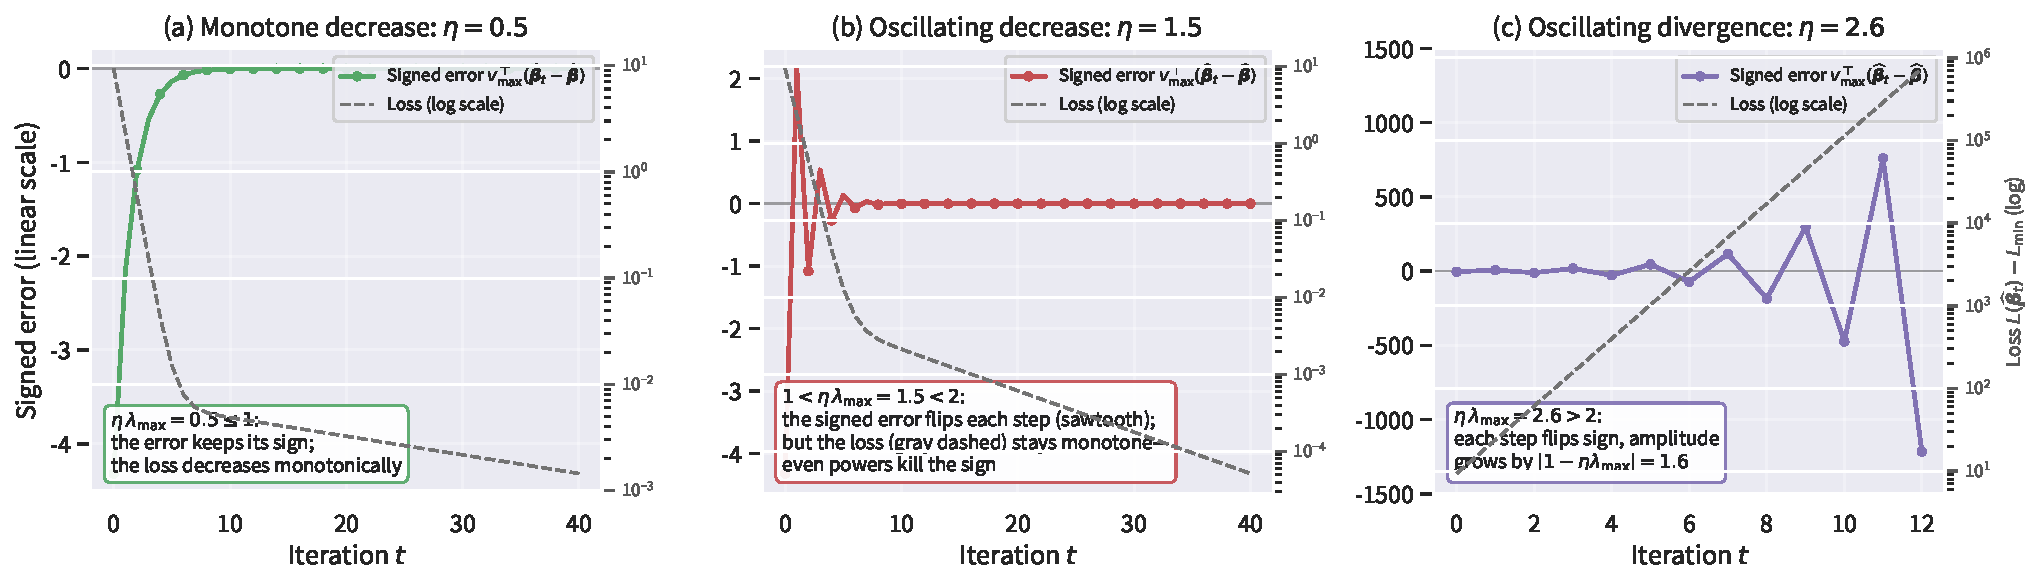
\includegraphics[width=\linewidth]{figures/ch4_loss.pdf}
  \caption{The three regimes of the signed error (colored solid lines, left axis, linear scale) and the loss (gray dashed, right axis, log scale) versus iteration count $t$ — same quadratic problem, same initialization, only $\eta$ varies: (a) monotone descent — $\eta\lambda_{\max} \le 1$, the largest-eigenvalue signed error never changes sign and the loss is monotone; (b) oscillating descent — $1 < \eta\lambda_{\max} < 2$, the signed error flips sign every step into a sawtooth, yet the loss, being an even power of the error factors, keeps decreasing monotonically; (c) oscillation without convergence — $\eta\lambda_{\max} > 2$, the error flips sign every step with amplitude growing by $|1-\eta\lambda_{\max}|$, and the loss explodes.}
  \label{fig:ch4-loss}
\end{figure}

Two practical corollaries, both fragments of the answer to ``why study linear regression'':

\begin{itemize}
  \item \textbf{The condition number rules everything.} When $\kappa \approx 1$ (eigen-directions of similar length), $\rho^\star \approx 0$ and convergence takes a handful of steps; when $\kappa \gg 1$ (the ill-conditioning of Section~\ref{sec:hd-break}), $\rho^\star \approx 1 - 2/\kappa$ and convergence needs $O(\kappa \log(1/\varepsilon))$ steps — \textit{the engineering folklore ``standardize your features first''} is here half a theorem: standardization normalizes the diagonal of $\X^\top\X$ and \textbf{removes the part of the condition number due to units} --- but eigenvalue spread caused by \textbf{correlation structure} (collinearity) is untouched, and $\kappa$ can still be large.
  \item \textbf{Preconditioning $=$ GD in better coordinates.} Whitening after a spectral decomposition of $\X^\top\X$ is equivalent to running gradient descent in a better coordinate system; conjugate gradients (CG) can be viewed as ``GD with an automatically chosen step size and direction at every step,'' reaching $\bhat$ \textbf{exactly} in $d$ steps (finite termination for quadratic functions). From GD to CG to direct inversion is one family: the two ends are ``iterate $t$ steps'' and ``one closed-form step,'' and everything in between is an interpolation of the same geometry.
\end{itemize}

\begin{figure}[htbp]
  \centering
  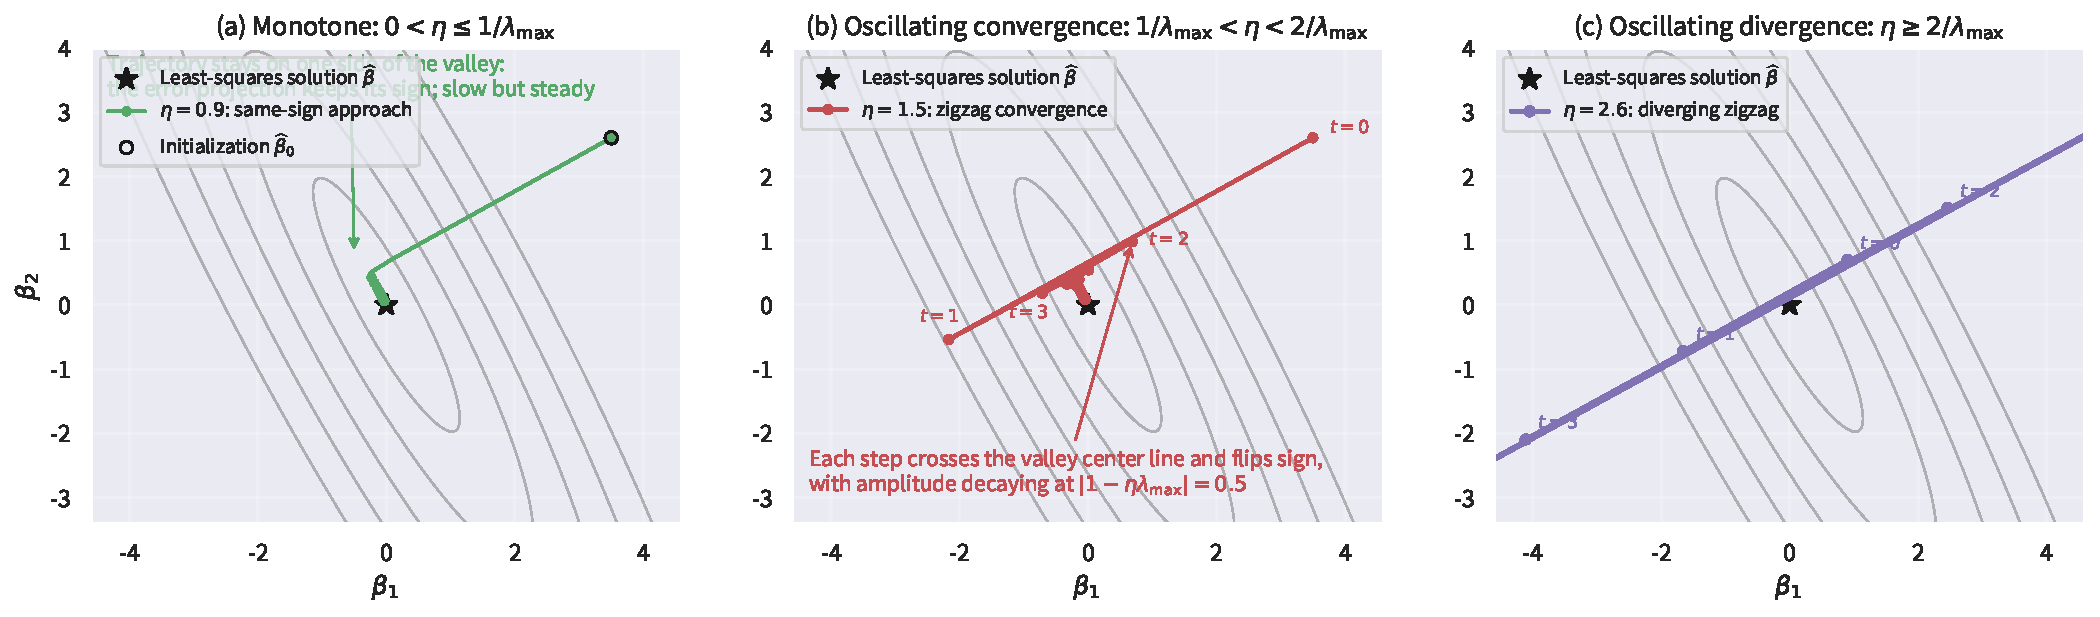
\includegraphics[width=\linewidth]{figures/ch4_gd.pdf}
  \caption{Three trajectories of gradient descent on a quadratic loss (an elliptical valley with condition number $\kappa = 25$), one per step-size regime: (a) $\eta = 0.9 \le 1/\lambda_{\max}$ — the trajectory never crosses the valley floor, approaching without sign flips, but crawls slowly along the ``thin'' direction; (b) $1/\lambda_{\max} < \eta = 1.5 < 2/\lambda_{\max}$ — the trajectory crosses the valley floor and flips sign every step, the zigzag amplitude decaying by $|1-\eta\lambda_{\max}| = 0.5$ — oscillating descent; (c) $\eta = 2.6 > 2/\lambda_{\max}$ — every step flips sign with amplitude growing by $1.6$, flying out of view within a few steps.}
  \label{fig:ch4-gd}
\end{figure}

\subsection{A Side-by-Side Comparison with the Closed-Form Solution}

\begin{center}
\resizebox{\textwidth}{!}{%
\begin{tabular}{@{}lll@{}}
\toprule
 & Closed form $\bhat = (\X^\top\X)^{-1}\X^\top\y$ & Gradient descent \eqref{eq:gd} \\
\midrule
Character & One shot (solves a $d\times d$ system) & Successive approximation, error $\propto \rho^t$ after $t$ steps \\
Cost (full column rank) & $O(nd^2 + d^3)$; must form $\X^\top\X$ & $O(nd)$ matrix-vector products per step; memory-friendly \\
Applicable regime & The classical region $n \gg d$ & Any $n, d$ (with regularization / early stopping) \\
Ill-conditioning $\kappa \gg 1$ & Numerically unstable (squared condition number) & Painfully slow convergence (the same $\kappa$, a different disease) \\
Relation to $\bhat$ & It \emph{is} $\bhat$ & Its fixed point is $\bhat$; $\widehat{\bbeta}_t$ has the exact solution \eqref{eq:gd-exact} \\
\bottomrule
\end{tabular}}
\end{center}

\begin{keybox}[Chapter takeaways]
\begin{itemize}
  \item The fixed-point condition $\nabla L = \zero$ of the iteration $\widehat{\bbeta}_{t+1} = \widehat{\bbeta}_t - \eta\,\X^\top(\X\widehat{\bbeta}_t - \y)$ \emph{is} the normal equation; the unique fixed point is the closed-form solution $\bhat$ — the optimization and the algebraic views end at the same place;
  \item Combining the two formulas yields the exact solution $\widehat{\bbeta}_t = \bhat + (\bm{I} - \eta\X^\top\X)^t(\widehat{\bbeta}_0 - \bhat)$: the error is multiplied by $\bm{I} - \eta\X^\top\X$ each step, and the eigenvalues $1 - \eta\lambda_j$ govern the decay direction by direction;
  \item Convergence requires $0 < \eta < 2/\lambda_{\max}$; the optimal $\eta^\star = 2/(\lambda_{\min} + \lambda_{\max})$ has rate $(\kappa - 1)/(\kappa + 1)$ — ``standardize your features'' removes unit-driven ill-conditioning (correlation-driven ill-conditioning it cannot fix);
  \item The geometric-series form shows GD assembling $(\X^\top\X)^{-1}$ by a degree-$t$ polynomial: the closed form hands over the inverse, the iteration pays it in installments; conjugate gradients is the midpoint of the family.
\end{itemize}
\end{keybox}

\begin{exercise}\label{ex:gd-rate}
From \eqref{eq:gd-exact}, derive: if $\widehat{\bbeta}_0 = \zero$ and $\eta = \eta^\star$, then $\norm{\widehat{\bbeta}_t - \bhat} \le \big(\frac{\kappa-1}{\kappa+1}\big)^t \norm{\bhat}$; and from this, give a big-$O$ expression for the number of steps needed to reach $\norm{\widehat{\bbeta}_t - \bhat} \le \varepsilon$.
\end{exercise}

\begin{exercise}\label{ex:neumann}
Verify the identity $\eta\sum_{k=0}^{t-1}(\bm{I} - \eta\X^\top\X)^k \X^\top\y = \big[\bm{I} - (\bm{I} - \eta\X^\top\X)^t\big]\bhat$ (hint: multiply both sides by $\X^\top\X$, or use the Neumann series), and explain why it is precisely the left-multiplied form of \eqref{eq:gd-exact-zero}.
\end{exercise}
